\documentclass{beamer}
\usepackage[utf8]{inputenc}
\usepackage{algorithm,algorithmic}
\usepackage{amsmath}
\usepackage{amssymb}
\usepackage{mathtools}
\usepackage{amsthm}

\def\E{\mathbb{E}}
\newcommand{\bx}{\mathbf{x}} 
\newcommand{\by}{\mathbf{y}} 

\usetheme{Madrid}
\usecolortheme{beaver}

\def\reals{\mathbb{R}}

\begin{document}

\begin{frame}

{\Large
A12:Tackling Distribution Shifts via Test-Time Adaptation and Optimization
}
\\
Instructor: Jun-Kun Wang (Assistant Professor at ECE and HDSI)
\end{frame}


\begin{frame}{Training is Optimization}

Supervised learning
\begin{itemize}
\item $n$ observations: $\left(x_i \in \reals^d, y_i \in \{-1,+1\} \right)$, $i=1,\dots, n$.
\item Prediction function: $h(x_i; w) \in \reals$ parametrized by $w \in W$. 
\end{itemize}
{
\centering
 \includegraphics[width=10cm]{catdog.jpg}
% \includegraphics[0.2\textwidth]{catdog.jpg}
}

\pause 

\begin{exampleblock}{Regularized Empirical Risk}
$\min_{w \in W} \, \underbrace{ \frac{1}{n} \sum_{i=1}^n \ell( x_i, y_i; h(x_i;w) ) }_{ \text{Empirical Risk} } +  \underbrace{ \lambda \phi( w ) }_{ \text{Regularization} }$
\end{exampleblock}

\end{frame}


\begin{frame}

{\Large
Mathematical Background and Gradient Flow
}
\end{frame}


\begin{frame}{Review: Calculus}

\Large 
(\textbf{Derivative}) For a function $g(\cdot): \reals \to \reals$ and $x \in \reals$,
consider
\begin{align*}
    \lim_{\delta \to 0} \frac{g(x+\delta) - g(x)}{\delta}.
\end{align*}

\pause

\begin{block}{}
The function $g(\cdot)$ is said to be ``differentiable'' if this limit exits for all $x \in \reals$. In that case, the limit is called the ``derivative'' of $g(\cdot)$.
\end{block}

\end{frame}


\begin{frame}{Review: Calculus}

\Large 
(\textbf{Derivative}) For a function $g(\cdot): \reals \to \reals$ and $x \in \reals$,
consider
\begin{align*}
    \lim_{\delta \to 0} \frac{g(x+\delta) - g(x)}{\delta}.
\end{align*}

We denote the derivative as
\begin{alertblock}{}
\hfill \break
\hfill \break
\end{alertblock}

\end{frame}

\begin{frame}{Review: Calculus}

\Large 

(\textbf{Gradient}) For a differentiable function $f: \reals^d \to \reals$ and $\mathbf{x} \in \reals^d$, 
the gradient is 
\begin{align*}
    \nabla f(\mathbf{x}) = \begin{bmatrix} \frac{\partial f}{\partial x_1} \\ \frac{\partial f}{\partial x_2} \\ \vdots \\ \frac{\partial f}{\partial x_d} \end{bmatrix},
\end{align*}
where
\begin{align*}
    \frac{\partial f}{\partial x_1} = \lim_{\delta \to 0} \frac{f(x_1+\delta; x_2 ; \ldots ; x_d ) - f(x_1 ; x_2 ; \ldots ; x_d )}{\delta}.
\end{align*}


\end{frame}

\begin{frame}{Review: Calculus}
\Large 
\begin{definition}
(\textbf{Hessian}) For a twice continuously differentiable function $f: \reals^d \to \reals$ and $\mathbf{x} \in \reals^d$, the Hessian matrix of $f(\cdot)$ at $\mathbf{x}$ is defined by
$$
 \nabla^2f(\mathbf{x})= \begin{bmatrix} \frac{\partial^2 f}{\partial x_1^2} & \frac{\partial^2 f}{\partial x_1 \partial x_2} & \cdots & \frac{\partial^2 f}{\partial x_1 \partial x_d} \\ \frac{\partial^2 f}{\partial x_2 \partial x_1} & \frac{\partial^2 f}{\partial x_2^2} & \cdots & \frac{\partial^2 f}{\partial x_2 \partial x_d} \\ \vdots & \vdots & \ddots & \vdots \\ \frac{\partial^2 f}{\partial x_d \partial x_1} & \frac{\partial^2 f}{\partial x_d \partial x_2} & \cdots & \frac{\partial^2 f}{\partial x_d^2} \end{bmatrix} \in \reals^{d \times d}
$$
\end{definition}



\end{frame}


\begin{frame}{Exercise}

\Large 
Let $f : \reals^2 \to \reals $ be defined by $f(\mathbf{x}) = x_1^2 x_2$. Then
\begin{block}{}
%\begin{align*}
 $   \nabla f(\mathbf{x}) = $
    %\begin{bmatrix}
    %    2x_1 x_2 \\ x_1^2
    %\end{bmatrix} \in \reals^2,
%\end{align*}
\hfill \break
\end{block}
and 
\begin{alertblock}{}
%\begin{align*}
 $   \nabla^2 f(\mathbf{x}) = $
%    \begin{bmatrix}
%        2x_2 & 2x_1 \\ 2x_1 & 0
%    \end{bmatrix} \in \reals^{2 \times 2}.
%\end{align*}
\hfill \break
\hfill \break
\end{alertblock}



\end{frame}


\begin{frame}

\Large 

Convergence Rate

\end{frame}

\begin{frame}{}

\Large

Finding the minimizer of a function 

\begin{equation}
\min_{x \in \reals^d} f(x)
\end{equation}


{
\centering
 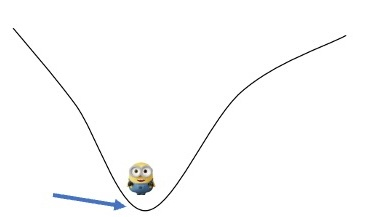
\includegraphics[width=7cm]{minimal.jpg}
}


\end{frame}

\begin{frame}{Optimality Gap}

\begin{definition}
(\textbf{Optimality Gap}): Given a function $f$ such that $f: \reals^d \to \reals$, the optimality gap is the difference between the value of $f$ at $\mathbf{x}_k \in \reals^d$ at some time point $k$ and the optimal value, i.e.
\begin{align*}
    f(\mathbf{x}_k) - \min_{\mathbf{x}} f(\mathbf{x})% = f(\mathbf{x}_k) - f_\ast, 
\end{align*}
%where
%\begin{align*}
%    f_\ast :=  \min_{\mathbf{x}} f(\mathbf{x}).
%\end{align*}
\end{definition}


\end{frame}




\begin{frame}{Gradient Descent}
\Large 
$\min_{x \in \reals^d} f(x)$. 

\begin{algorithm}[H]
\begin{algorithmic}[1]
\Large 
%\caption{\textsc{Gradient Descent}
%} \label{alg:GD}{}
\STATE Input: an initial point $\mathbf{x}_{0} \in \textbf{dom }f$ and step size $\eta$.
\FOR{$k=1$ to $K$}
\STATE $\mathbf{x}_{k+1} \leftarrow \mathbf{x}_{k} - \eta \nabla f \left( \mathbf{x_{k}} \right)$
\ENDFOR
\STATE Return $\mathbf{x}_{k+1}$.
\end{algorithmic}
\end{algorithm}


\end{frame}


\begin{frame}{}

\Large 
(\textbf{Gradient Flow}): 
Let $f: \reals^d \to \reals$ be a smooth function. Gradient flow is a smooth curve $\mathbf{x}: \reals \to \reals^d$ such that
\begin{align*}
    &\frac{d\mathbf{x}(t)}{dt} = - \nabla f \left( \mathbf{x}(t) \right) 
    % & \mathbf{x}(0) = \mathbf{x}_0
\end{align*}

\end{frame}

\begin{frame}{Gradient Flow is Gradient Descent as $\eta \rightarrow 0$}

\end{frame}

\begin{frame}{}

\end{frame}

\begin{frame}{}

\end{frame}

\begin{frame}

\begin{block}{}
Our project: \\ Tackling Distribution Shifts via Test-Time Adaptation and Optimization
\end{block}

\end{frame}

\begin{frame}
{
\centering
 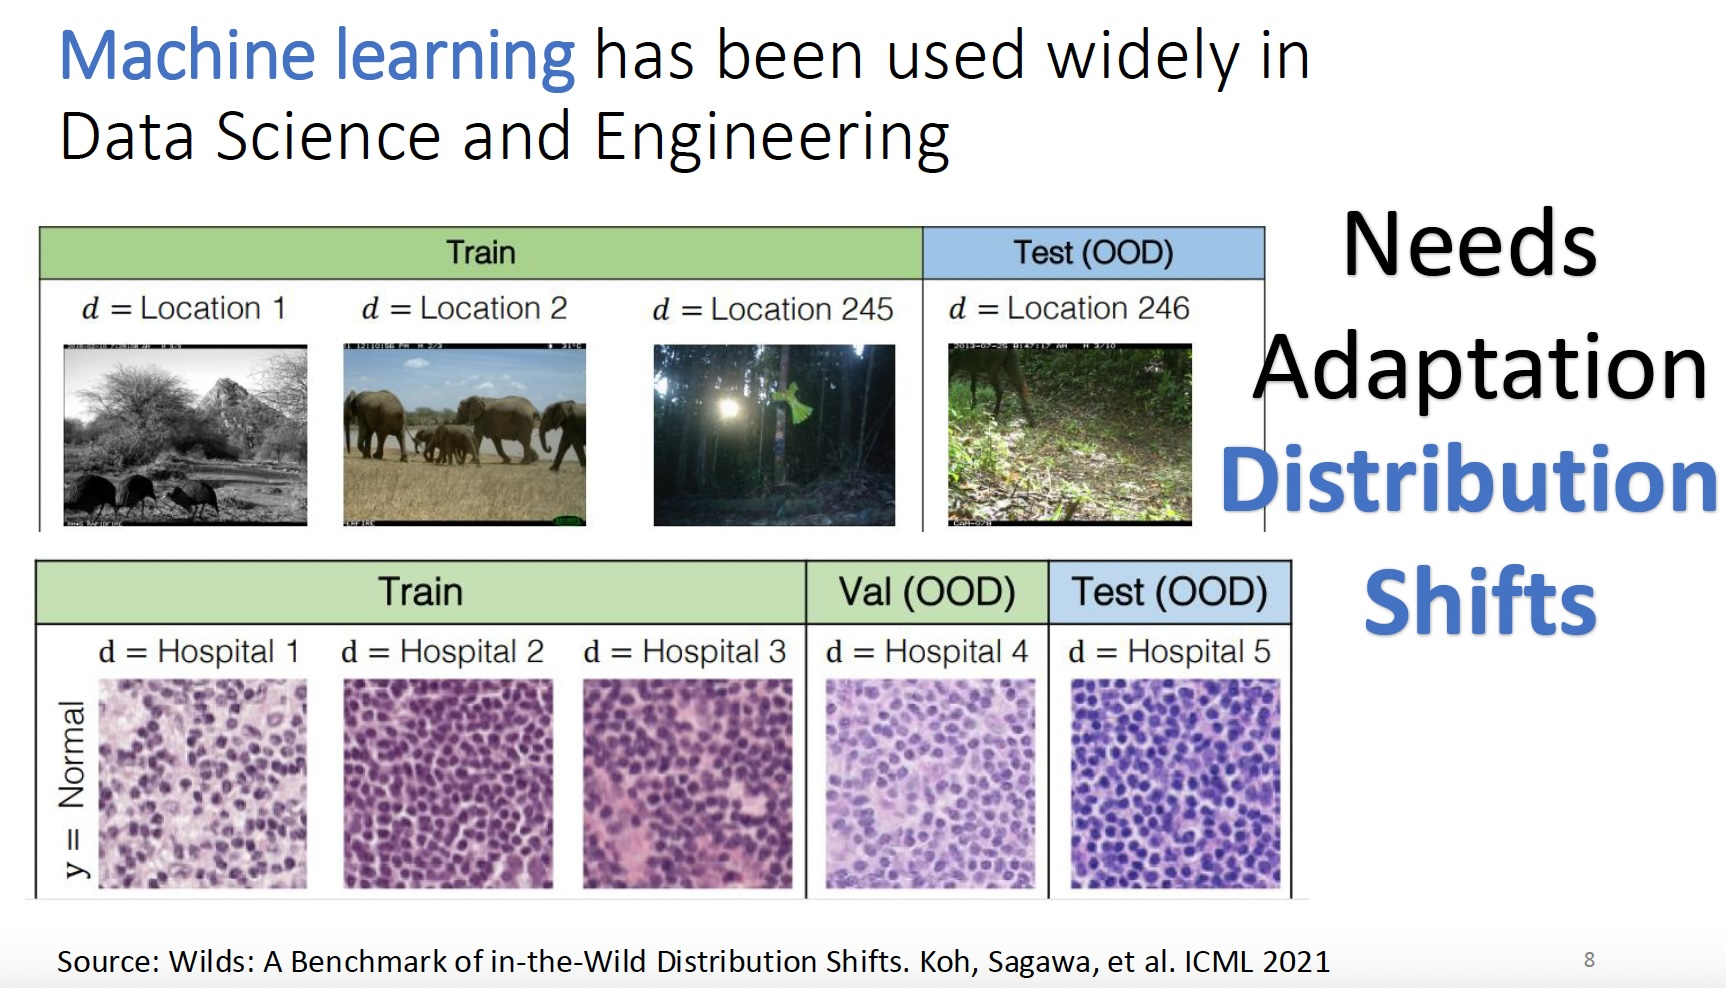
\includegraphics[width=12cm]{fig1.jpg}
}


\end{frame}

\begin{frame}[t]
\large 
\begin{exampleblock}{}
Given a source model, adapt the model to a new domain, by using un-labeled samples of data from the new domain.
\end{exampleblock}

\end{frame}

\begin{frame}[t]

{
\centering
 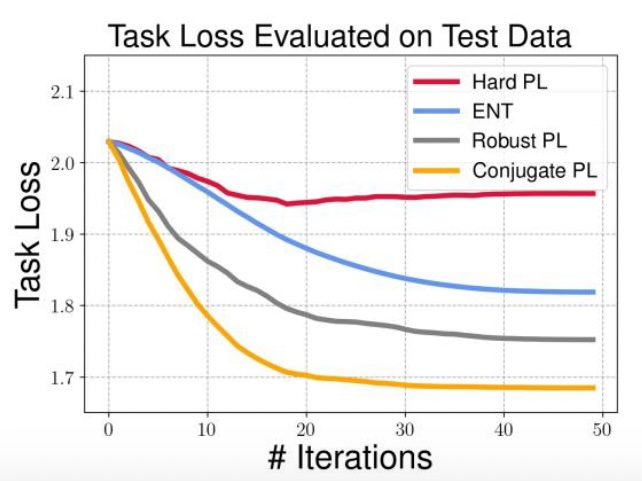
\includegraphics[width=12cm]{fig3.jpg}
}

\end{frame}

\begin{frame}[t]
{}


Research Group Meeting Schedule

\url{https://docs.google.com/document/d/1nEa5PQowFBSJhRoUYPjrQ-NKL4G6Qz5VCiv8AjwMQCc/edit}

\end{frame}


\end{document}

